\section{Рабочий проект}
\subsection{Спецификация разработанных класов и компонентов}

В результате разработки программного продукта были реализованы классы и компоненты, обеспечивающие работоспособность системы. Спецификация классов и компонентов описана в данной главе.

\subsubsection{Спецификация класса ArtistController}
Данный класс является контроллером, обрабатывающим запросы,связанные с артистами. Описание класса представлено в таблице \ref{classArtist:table}

\renewcommand{\arraystretch}{0.8} % уменьшение расстояний до сетки таблицы
\begin{xltabular}{\textwidth}{|X|p{2.5cm}|>{\setlength{\baselineskip}{0.7\baselineskip}}p{4.85cm}|>{\setlength{\baselineskip}{0.7\baselineskip}}p{4.85cm}|}
	\caption{Описание класса ArtistController\label{classArtist:table}}\\
	\hline \centrow \setlength{\baselineskip}{0.7\baselineskip} Название поля(метода) & \centrow \setlength{\baselineskip}{0.7\baselineskip} Область видимости & \centrow Тип значения & \centrow Описание \\
	\hline \centrow 1 & \centrow 2 & \centrow 3 & \centrow 4\\ \hline
	\endfirsthead
	\continuecaption{Продолжение таблицы\ref{classArtist:table}}
	\hline \centrow 1 & \centrow 2 & \centrow 3 & \centrow 4\\ \hline
	\finishhead
	artistService & private & ArtistService & Объект, отвечающий за бизнес-логику сущности "<Artist"> \\
	\hline albumService & private & AlbumService & Объект, отвечающий за бизнес-логику сущности "<Album"> \\
	\hline getArtist ById & public & ResponseEntity <ArtistDto> & Возвращает артиста по идентификатору. Входные параметры: id - идентификатор артиста \\
	\hline getArtist Albums & public & ResponseEntity <ArtistDto> & Возвращает артиста со списком альбомов по идентификатору. Входные параметры: id - идентификатор артиста 
\end{xltabular}
\renewcommand{\arraystretch}{1.0} % восстановление сетки


\subsubsection{Спецификация класса AlbumController}
Данный класс является контроллером, обрабатывающим запросы, связанные с альбомами. Описание класса представлено в таблице \ref{classAlbum:table}

\begin{xltabular}{\textwidth}{|X|p{2.5cm}|>{\setlength{\baselineskip}{0.7\baselineskip}}p{4.85cm}|>{\setlength{\baselineskip}{0.7\baselineskip}}p{4.85cm}|}
	\caption{Описание класса AlbumController}\label{classAlbum:table}\\
	\hline \centrow \setlength{\baselineskip}{0.7\baselineskip} Название поля(метода) & \centrow \setlength{\baselineskip}{0.7\baselineskip} Область видимости & \centrow Тип значения & \centrow Описание \\
	\hline \centrow 1 & \centrow 2 & \centrow 3 & \centrow 4\\ \hline
	\endfirsthead
	\continuecaption{Продолжение таблицы \ref{classAlbum:table}}
	\hline \centrow 1 & \centrow 2 & \centrow 3 & \centrow 4\\ \hline
	\finishhead
	albumService & private & AlbumService & Объект, отвечающий за бизнес-логику сущности "<Album"> \\
	\hline trackService & private & TrackService & Объект, отвечающий за бизнес-логику сущности "<Track"> \\
	\hline getAlbum ById & public & ResponseEntity <AlbumDto> & Возвращает альбом по идентификатору. Входные параметры: id - идентификатор альбома 
\end{xltabular}

\subsubsection{Спецификация класса PlaylistController}
Данный класс является контроллером, обрабатывающим запросы, связанные с плейлистами. Описание класса представлено в таблице \ref{classPlaylist:table}.

\begin{xltabular}{\textwidth}{|X|p{2.5cm}|>{\setlength{\baselineskip}{0.7\baselineskip}}p{4.83cm}|>{\setlength{\baselineskip}{0.7\baselineskip}}p{4.85cm}|}
	\caption{Описание класса PlaylistController}\label{classPlaylist:table}\\
	\hline \centrow \setlength{\baselineskip}{0.7\baselineskip} Название поля(метода) & \centrow \setlength{\baselineskip}{0.7\baselineskip} Область видимости & \centrow Тип значения & \centrow Описание \\
	\hline \centrow 1 & \centrow 2 & \centrow 3 & \centrow 4\\ \hline
	\endfirsthead
	\continuecaption{Продолжение таблицы \ref{classPlaylist:table}}
	\hline \centrow 1 & \centrow 2 & \centrow 3 & \centrow 4\\ \hline
	\finishhead
	playlist Service & private & PlaylistService & Объект, отвечающий за бизнес-логику сущности "<Playlist"> \\
	\hline getPlaylist Info & public & ResponseEntity <PlaylistDetailsDto> & Возвращает информацию о плейлисте по идентификатору. Входные параметры: id - идентификатор плейлиста \\
	\hline getPlaylist Tracklist & public & ResponseEntity <PlaylistTracklistDto> & Возвращает список треков плейлиста по идентификатору. Входные параметры: id - идентификатор плейлиста \\
	\hline createNew Playlist & public & ResponseEntity <PlaylistCreatedDto> & Создает новый плейлист. Входные параметры: newPlaylist - объект, содержащий данные нового плейлиста \\
	\hline deletePlaylist & public & ResponseEntity <?> & Удаляет плейлист по идентификатору. Входные параметры: id - идентификатор плейлиста \\
	\hline addTracksTo Playlist & public & ResponseEntity <?> & Добавляет треки в плейлист по идентификатору. Входные параметры: id - идентификатор плейлиста, tracks - объект, содержащий список идентификаторов треков \\
	\hline removeTracks FromPlaylist & public & ResponseEntity <PlaylistTracklistDto> & Удаляет треки из плейлиста по идентификатору. Входные параметры: id - идентификатор плейлиста, tracks - объект, содержащий список идентификаторов треков \\
	\hline updatePlaylist Details & public & ResponseEntity <PlaylistDetailsDto> & Обновляет детали плейлиста по идентификатору. Входные параметры: id - идентификатор плейлиста, newDetails - объект, содержащий новые данные плейлиста 
\end{xltabular}

\subsubsection{Спецификация класса TrackController}
Данный класс является контроллером, обрабатывающим запросы, связанные с плейлистами. Описание класса представлено в таблице \ref{classTrack:table}.

\renewcommand{\arraystretch}{0.8} % уменьшение расстояний до сетки таблицы
\begin{xltabular}{\textwidth}{|X|p{2.5cm}|>{\setlength{\baselineskip}{0.7\baselineskip}}p{4.83cm}|>{\setlength{\baselineskip}{0.7\baselineskip}}p{4.85cm}|}
	\caption{Описание класса TrackController}\label{classTrack:table}\\
	\hline \centrow \setlength{\baselineskip}{0.7\baselineskip} Название поля(метода) & \centrow \setlength{\baselineskip}{0.7\baselineskip} Область видимости & \centrow Тип значения & \centrow Описание \\
	\hline \centrow 1 & \centrow 2 & \centrow 3 & \centrow 4\\ \hline
	\endfirsthead
	\continuecaption{Продолжение таблицы \ref{classTrack:table}}
	\hline \centrow 1 & \centrow 2 & \centrow 3 & \centrow 4\\ \hline
	\finishhead
	trackService & private & TrackService & Объект, отвечающий за бизнес-логику сущности "<Track"> \\
	\hline isTrackExists & public & ResponseEntity <BooleanResponse> & Проверяет существование трека по идентификатору. Входные параметры: id - идентификатор трека \\
\end{xltabular}
\renewcommand{\arraystretch}{1.0}

\subsubsection{Спецификация класса UserManagementController}
Данный класс является контроллером, обрабатывающим запросы, связанные с пользователем. Описание класса представлено в таблице \ref{classUsers:table}.

\renewcommand{\arraystretch}{0.8} % уменьшение расстояний до сетки таблицы
\begin{xltabular}{\textwidth}{|X|p{2.5cm}|>{\setlength{\baselineskip}{0.7\baselineskip}}p{4.83cm}|>{\setlength{\baselineskip}{0.7\baselineskip}}p{4.85cm}|}
	\caption{Описание класса UserManagementController}\label{classUsers:table}\\
	\hline \centrow \setlength{\baselineskip}{0.7\baselineskip} Название поля(метода) & \centrow \setlength{\baselineskip}{0.7\baselineskip} Область видимости & \centrow Тип значения & \centrow Описание \\
	\hline \centrow 1 & \centrow 2 & \centrow 3 & \centrow 4\\ \hline
	\endfirsthead
	\continuecaption{Продолжение таблицы \ref{classUsers:table}}
	\hline \centrow 1 & \centrow 2 & \centrow 3 & \centrow 4\\ \hline
	\finishhead
	userManage mentService & private & UserManagement Service & Объект, отвечающий за бизнес-логику управления пользователями \\
	\hline getUserBy Username & public & ResponseEntity <User> & Возвращает пользователя по имени пользователя. Входные параметры: username - имя пользователя \\
	\hline getUserBy Email & public & ResponseEntity <User> & Возвращает пользователя по адресу электронной почты. Входные параметры: email - адрес электронной почты пользователя \\
	\hline getUserById & public & ResponseEntity <PublicUserDto> & Возвращает пользователя по идентификатору. Входные параметры: id - идентификатор пользователя \\
	\hline createUser & public & ResponseEntity <?> & Создает нового пользователя. Входные параметры: user - объект, содержащий данные нового пользователя \\
	\hline deleteUser & public & ResponseEntity <?> & Удаляет пользователя по идентификатору. Входные параметры: id - идентификатор пользователя 
\end{xltabular}
\renewcommand{\arraystretch}{1.0}

\subsubsection{Спецификация класса TrackStorageContoller}
Данный класс является сервисом, обрабатывающим бизнес-логику, связанную с управлением пользователями. Описание класса представлено в таблице \ref{classStorage:table}.

\renewcommand{\arraystretch}{0.8} % уменьшение расстояний до сетки таблицы
\begin{xltabular}{\textwidth}{|X|p{2.5cm}|>{\setlength{\baselineskip}{0.7\baselineskip}}p{4.83cm}|>{\setlength{\baselineskip}{0.7\baselineskip}}p{4.85cm}|}
	\caption{Описание класса TrackController}\label{classStorage:table}\\
	\hline \centrow \setlength{\baselineskip}{0.7\baselineskip} Название поля(метода) & \centrow \setlength{\baselineskip}{0.7\baselineskip} Область видимости & \centrow Тип значения & \centrow Описание \\
	\hline \centrow 1 & \centrow 2 & \centrow 3 & \centrow 4\\ \hline
	\endfirsthead
	\continuecaption{Продолжение таблицы \ref{classStorage:table}}
	\hline \centrow 1 & \centrow 2 & \centrow 3 & \centrow 4\\ \hline
	\finishhead
	audioStream Loader & private & AudioStream Loader & Объект, отвечающий за организацию потока аудио \\
	\hline getTrack & public & ResponseEntity <StreamingResponseBody> & Метод, отвечающий за передачу частей аудио. Входные параметры: id - идентификатор трека\\
\end{xltabular}
\renewcommand{\arraystretch}{1.0}

\subsubsection{Спецификация класса ArtistService}
Данный класс обеспечивает бизнес-логику, связанную с исполнителями. Описание класса представлено в таблице \ref{classArtistService:table}.

\renewcommand{\arraystretch}{0.8} % уменьшение расстояний до сетки таблицы
\begin{xltabular}{\textwidth}{|X|p{2.5cm}|>{\setlength{\baselineskip}{0.7\baselineskip}}p{4.83cm}|>{\setlength{\baselineskip}{0.7\baselineskip}}p{4.85cm}|}
	\caption{Описание класса ArtistService}\label{classArtistService:table}\\
	\hline \centrow \setlength{\baselineskip}{0.7\baselineskip} Название поля(метода) & \centrow \setlength{\baselineskip}{0.7\baselineskip} Область видимости & \centrow Тип значения & \centrow Описание \\
	\hline \centrow 1 & \centrow 2 & \centrow 3 & \centrow 4\\ \hline
	\endfirsthead
	\continuecaption{Продолжение таблицы \ref{classArtistService:table}}
	\hline \centrow 1 & \centrow 2 & \centrow 3 & \centrow 4\\ \hline
	\finishhead
	artistsRepo sitory & private & ArtistsRepository & Репозиторий, отвечающий за доступ к данным артистов \\
	\hline getArtist ById & public & Optional <ArtistDto> & Возвращает артиста по идентификатору. Входные параметры: id - идентификатор артиста \\
	\hline getArtist WithAlbums & public & Optional <ArtistDto> & Возвращает артиста с альбомами по идентификатору. Входные параметры: id - идентификатор артиста 
\end{xltabular}
\renewcommand{\arraystretch}{1.0}

\subsubsection{Спецификация класса AlbumService}
Данный класс является сервисом, обрабатывающим бизнес-логику, связанную с альбомами. Описание класса представлено в таблице \ref{classAlbumService:table}.

\renewcommand{\arraystretch}{0.8} % уменьшение расстояний до сетки таблицы
\begin{xltabular}{\textwidth}{|X|p{2.5cm}|>{\setlength{\baselineskip}{0.7\baselineskip}}p{4.83cm}|>{\setlength{\baselineskip}{0.7\baselineskip}}p{4.85cm}|}
	\caption{Описание класса AlbumService}\label{classAlbumService:table}\\
	\hline \centrow \setlength{\baselineskip}{0.7\baselineskip} Название поля(метода) & \centrow \setlength{\baselineskip}{0.7\baselineskip} Область видимости & \centrow Тип значения & \centrow Описание \\
	\hline \centrow 1 & \centrow 2 & \centrow 3 & \centrow 4\\ \hline
	\endfirsthead
	\continuecaption{Продолжение таблицы \ref{classAlbumService:table}}
	\hline \centrow 1 & \centrow 2 & \centrow 3 & \centrow 4\\ \hline
	\finishhead
	albumRepo sitory & private & AlbumRepository & Репозиторий, отвечающий за доступ к данным альбомов \\
	\hline findAlbum ById & public & Optional <Album> & Возвращает альбом по идентификатору. Входные параметры: id - идентификатор альбома \\
	\hline findArtist Albums & public & List <AlbumOfArtistPreviewDto> & Возвращает список альбомов по идентификатору артиста. Входные параметры: artistId - идентификатор артиста 
\end{xltabular}
\renewcommand{\arraystretch}{1.0}


\subsubsection{Спецификация класса PlaylistService}
Данный класс является сервисом, обрабатывающим бизнес-логику, связанную с плейлистами. Описание класса представлено в таблице \ref{classPlaylistService:table}.

\renewcommand{\arraystretch}{0.8} % уменьшение расстояний до сетки таблицы
\begin{xltabular}{\textwidth}{|X|p{2.5cm}|>{\setlength{\baselineskip}{0.7\baselineskip}}p{4.83cm}|>{\setlength{\baselineskip}{0.7\baselineskip}}p{4.85cm}|}
	\caption{Описание класса PlaylistService}\label{classPlaylistService:table}\\
	\hline \centrow \setlength{\baselineskip}{0.7\baselineskip} Название поля(метода) & \centrow \setlength{\baselineskip}{0.7\baselineskip} Область видимости & \centrow Тип значения & \centrow Описание \\
	\hline \centrow 1 & \centrow 2 & \centrow 3 & \centrow 4\\ \hline
	\endfirsthead
	\continuecaption{Продолжение таблицы \ref{classPlaylistService:table}}
	\hline \centrow 1 & \centrow 2 & \centrow 3 & \centrow 4\\ \hline
	\finishhead
	playlistRepo sitory & private & PlaylistRepository & Репозиторий, отвечающий за доступ к данным плейлистов \\
	\hline trackService & private & TrackService & Объект, отвечающий за бизнес-логику сущности "<Track"> \\
	\hline userManagement Client & private & UserManage mentClient & Объект, отвечающий за взаимодействие с сервисом управления пользователями \\
	\hline getTracksBy PlaylistId & public & Set <Track> & Возвращает треки плейлиста по идентификатору. Входные параметры: playlistId - идентификатор плейлиста \\
	\hline getPlaylist ById & public & Optional <Playlist> & Возвращает плейлист по идентификатору. Входные параметры: playlistId - идентификатор плейлиста \\
	\hline createNew Playlist & public & Long & Создает новый плейлист. Входные параметры: newPlaylist - объект, содержащий данные нового плейлиста \\
	\hline removePlay listById & public & void & Удаляет плейлист по идентификатору. Входные параметры: id - идентификатор плейлиста \\
	\hline getPlaylist DtoById & public & Optional <PlaylistDto> & Возвращает DTO плейлиста по идентификатору. Входные параметры: id - идентификатор плейлиста \\
	\hline addTracks ToPlaylist & public & PlaylistTrack listDto & Добавляет треки в плейлист. Входные параметры: id - идентификатор плейлиста, trackIds - идентификаторы треков \\
	\hline removeTracks FromPlaylist & public & PlaylistTrack listDto & Удаляет треки из плейлиста. Входные параметры: id - идентификатор плейлиста, trackIds - идентификаторы треков \\
	\hline getPlaylist InfoById & public & PlaylistDetailsDto & Возвращает информацию о плейлисте по идентификатору. Входные параметры: id - идентификатор плейлиста \\
	\hline getPlaylist Tracklist & public & PlaylistTrack listDto & Возвращает треклист плейлиста по идентификатору. Входные параметры: playlistId - идентификатор плейлиста 
\end{xltabular}
\renewcommand{\arraystretch}{1.0}


\subsubsection{Спецификация класса UserManagementService}
Данный класс является сервисом, обрабатывающим бизнес-логику, связанную с управлением пользователями. Описание класса представлено в таблице \ref{classUserManagementService:table}.

\renewcommand{\arraystretch}{0.8} % уменьшение расстояний до сетки таблицы
\begin{xltabular}{\textwidth}{|X|p{2cm}|>{\setlength{\baselineskip}{0.7\baselineskip}}p{4.5cm}|>{\setlength{\baselineskip}{0.7\baselineskip}}p{4.85cm}|}
	\caption{Описание класса UserManagementService}\label{classUserManagementService:table}\\
	\hline \centrow \setlength{\baselineskip}{0.7\baselineskip} Название поля(метода) & \centrow \setlength{\baselineskip}{0.7\baselineskip} Область видимости & \centrow Тип значения & \centrow Описание \\
	\hline \centrow 1 & \centrow 2 & \centrow 3 & \centrow 4\\ \hline
	\endfirsthead
	\continuecaption{Продолжение таблицы \ref{classUserManagementService:table}}
	\hline \centrow 1 & \centrow 2 & \centrow 3 & \centrow 4\\ \hline
	\finishhead
		userManage mentRepository & private & UserManagement Repository & Репозиторий, отвечающий за доступ к данным пользователей \\
		\hline findUser ById & public & Optional <User> & Возвращает пользователя по идентификатору. Входные параметры: id - идентификатор пользователя \\
		\hline findUserBy Username & public & Optional <User> & Возвращает пользователя по имени пользователя. Входные параметры: username - имя пользователя \\
		\hline findUser ByEmail & public & Optional <User> & Возвращает пользователя по адресу электронной почты. Входные параметры: email - адрес электронной почты пользователя \\
		\hline existsById & public & boolean & Проверяет существование пользователя по идентификатору. Входные параметры: userId - идентификатор пользователя \\
		\hline existsBy Username & public & boolean & Проверяет существование пользователя по имени пользователя. Входные параметры: username - имя пользователя \\
		\hline existsByEmail & public & boolean & Проверяет существование пользователя по адресу электронной почты. Входные параметры: email - адрес электронной почты пользователя \\
		\hline deleteUser & public & void & Удаляет пользователя по идентификатору. Входные параметры: userId - идентификатор пользователя \\
		\hline saveUser & public & User & Сохраняет пользователя. Входные параметры: user - объект пользователя
\end{xltabular}
\renewcommand{\arraystretch}{1.0}

\subsubsection{Спецификация класса AudioStreamLoader}
Данный класс отвечает за загрузку и стриминг аудиофайлов. Описание класса представлено в таблице \ref{classAudioStreamLoader:table}.

\renewcommand{\arraystretch}{0.8} % уменьшение расстояний до сетки таблицы
\begin{xltabular}{\textwidth}{|X|p{2cm}|>{\setlength{\baselineskip}{0.7\baselineskip}}p{4.5cm}|>{\setlength{\baselineskip}{0.7\baselineskip}}p{4.85cm}|}
	\caption{Описание класса AudioStreamLoader}\label{classAudioStreamLoader:table}\\
	\hline \centrow \setlength{\baselineskip}{0.7\baselineskip} Название поля(метода) & \centrow \setlength{\baselineskip}{0.7\baselineskip} Область видимости & \centrow Тип значения & \centrow Описание \\
	\hline \centrow 1 & \centrow 2 & \centrow 3 & \centrow 4\\ \hline
	\endfirsthead
	\continuecaption{Продолжение таблицы \ref{classAudioStreamLoader:table}}
	\hline \centrow 1 & \centrow 2 & \centrow 3 & \centrow 4\\ \hline
	\finishhead
	LOGGER & private& Logger & Логгер для класса AudioStreamLoader \\
	\hline s3Service & private & S3Service & Сервис для работы с S3-хранилищем \\
	\hline catalogClient & private & CatalogClient & Клиент для взаимодействия с каталогом \\
	\hline loadPartial MediaFrom Storage & private & StreamingResponse Result & Загружает часть медиафайла из хранилища. Входные параметры: bytes - массив байтов, startPos - начальная позиция, endPos - конечная позиция \\
	\hline loadPartial MediaFrom Storage & public & StreamingResponse Result & Загружает часть медиафайла из хранилища по идентификатору и значениям диапазона. Входные параметры: id - идентификатор файла, rangeValues - значения диапазона \\
	\hline loadEntire MediaFile & public & StreamingResponse Result & Загружает весь медиафайл из хранилища. Входные параметры: bytes - массив байтов 
\end{xltabular}
\renewcommand{\arraystretch}{1.0}

\subsubsection{Спецификация класса UserManagementClient}
Класс UserManagementClient предоставляет методы для взаимодействия с сервисом управления пользователями. Описание класса представлено в таблице \ref{classUserManagementClient:table}.

\renewcommand{\arraystretch}{0.8} % уменьшение расстояний до сетки таблицы
\begin{xltabular}{\textwidth}{|X|p{2cm}|>{\setlength{\baselineskip}{0.7\baselineskip}}p{4.5cm}|>{\setlength{\baselineskip}{0.7\baselineskip}}p{4.85cm}|}
	\caption{Описание класса UserManagementClient}\label{classUserManagementClient:table}\\
	\hline \centrow \setlength{\baselineskip}{0.7\baselineskip} Название поля(метода) & \centrow \setlength{\baselineskip}{0.7\baselineskip} Область видимости & \centrow Тип значения & \centrow Описание \\
	\hline \centrow 1 & \centrow 2 & \centrow 3 & \centrow 4\\ \hline
	\endfirsthead
	\continuecaption{Продолжение таблицы \ref{classUserManagementClient:table}}
	\hline \centrow 1 & \centrow 2 & \centrow 3 & \centrow 4\\ \hline
	\finishhead
	userManagement Name & private & String & Имя сервиса управления пользователями, получаемое из конфигурации \\
	\hline discovery Client & private final & DiscoveryClient & Клиент для обнаружения сервисов \\
	\hline restTemplate & private final & RestTemplate & Шаблон для выполнения HTTP-запросов \\
	\hline getUserManage mentUri & private & String & Получает URI сервиса управления пользователями. Выбрасывает IllegalStateException, если сервис недоступен \\
	\hline isUserExists & public & BooleanResponse & Проверяет существование пользователя по идентификатору. Входные параметры: userId - идентификатор пользователя. Выбрасывает UserNotFoundException при отсутствии пользователя \\
	\hline getUserPreview & public & OwnerPreviewDto & Получает превью информации о пользователе по идентификатору. Входные параметры: id - идентификатор пользователя. Выбрасывает UserNotFoundException при отсутствии пользователя 
\end{xltabular}
\renewcommand{\arraystretch}{1.0}

\subsubsection{Спецификация класса DiscoveryClientUtil}
Класс DiscoveryClientUtil предоставляет утилитарные методы для взаимодействия с сервисами через DiscoveryClient. Описание класса представлено в таблице \ref{classDiscoveryClientUtil:table}.

\renewcommand{\arraystretch}{0.8} % уменьшение расстояний до сетки таблицы
\begin{xltabular}{\textwidth}{|X|p{2cm}|>{\setlength{\baselineskip}{0.7\baselineskip}}p{4.5cm}|>{\setlength{\baselineskip}{0.7\baselineskip}}p{4.85cm}|}
	\caption{Описание класса DiscoveryClientUtil}\label{classDiscoveryClientUtil:table}\\
	\hline \centrow \setlength{\baselineskip}{0.7\baselineskip} Название поля(метода) & \centrow \setlength{\baselineskip}{0.7\baselineskip} Область видимости & \centrow Тип значения & \centrow Описание \\
	\hline \centrow 1 & \centrow 2 & \centrow 3 & \centrow 4\\ \hline
	\endfirsthead
	\continuecaption{Продолжение таблицы \ref{classDiscoveryClientUtil:table}}
	\hline \centrow 1 & \centrow 2 & \centrow 3 & \centrow 4\\ \hline
	\finishhead
	discoveryClient & private final & DiscoveryClient & Клиент для обнаружения сервисов \\
	\hline DiscoveryClient Util & protected & Конструктор & Инициализирует DiscoveryClientUtil с использованием переданного DiscoveryClient \\
	\hline getServiceUri & private & String & Получает URI сервиса по его имени. Входные параметры: serviceName - имя сервиса. Выбрасывает IllegalStateException, если сервис недоступен
\end{xltabular}
\renewcommand{\arraystretch}{1.0}

\subsection{Тестирование программного продукта}

Для проверки работоспособности бизнес-логики разработанного программного продукта, было осуществлено модульное тестирование.
Тестирование является ключевым этапом разработки программного обеспечения, обеспечивающим его качество и надежность. Этот процесс включает в себя проверку и оценку программного продукта на соответствие заданным требованиям и ожиданиям пользователей. Цель тестирования заключается в выявлении дефектов, ошибок и несоответствий в программном коде до его выпуска в эксплуатацию, что позволяет минимизировать риски и затраты, связанные с исправлением проблем в будущем. 

\subsubsection{Модульное тестирование}
 
Модульное тестирование (или unit testing) является неотъемлемой частью процесса разработки программного обеспечения. Оно направлено на проверку правильности работы отдельных модулей программы, то есть её минимальных функциональных частей. Каждый модуль, как правило, представляет собой функцию или метод, который выполняет определённую задачу. Основная цель модульного тестирования — удостовериться, что каждый модуль функционирует корректно в соответствии с заданными спецификациями.
В процессе модульного тестирования создаются тестовые случаи, которые проверяют различные аспекты поведения модуля. Эти тестовые случаи могут включать проверку правильности выполнения функции при различных входных данных, оценку корректности обработки ошибок, проверку граничных условий и исключительных ситуаций. Тесты должны быть изолированными, то есть тестируемый модуль должен проверяться в контексте, который максимально исключает влияние других частей системы. Для этого часто используются заглушки (stubs) и моки (mocks) — вспомогательные объекты, заменяющие реальные зависимости модуля.
Для тестирования модуля частичной загрузки контента AudioStreamLoader были использованы библиотеки JUnit и Mockito.
JUnit — это библиотека для написания и выполнения тестов для языка Java. Она предоставляет аннотации для определения тестовых методов, методы для проверки условий и механизмы для организации и запуска тестов. JUnit позволяет разработчикам автоматически проверять корректность работы кода, что повышает надежность и качество программного обеспечения.
Mockito — это библиотека для создания мок-объектов, которые имитируют поведение реальных объектов в тестах. Это особенно полезно для тестирования компонентов, которые зависят от внешних систем или сложных взаимодействий. Mockito позволяет настроить возвращаемые значения, проверять вызовы методов и задавать ожидания, что облегчает написание изолированных и контролируемых тестов.

На рисунках \ref{unitASL:image}-\ref{unitASLentire:image} представлены листинги модульныех тестов для модуля частичной загрузки контента AudioStreamLoader.
\begin{figure}[ht]
\begin{lstlisting}[language=Java]
@ExtendWith(MockitoExtension.class)
public class AudioStreamLoaderTest {
	@Mock
	private S3Service s3Service;
	@Mock
	private RangeValuesUtils rangeValuesUtils;
	@InjectMocks
	private AudioStreamLoader audioStreamLoader;
	private byte[] sampleBytes;
	@BeforeEach
	public void setUp() {
		sampleBytes = new byte[]{1, 2, 3, 4, 5, 6, 7, 8, 9, 10};
	}
}
\end{lstlisting}  
\caption{Настрока модульных тестов класса AudioStreamLoader}
\label{unitASL:image}
\end{figure}
\begin{figure}[!ht]
	\begin{lstlisting}[language=Java]
		@Test
		public void NoRangeValues_LoadsEntireFile() throws Exception {
			Long id = 1L;
			when(s3Service.getTrackObject(id)).thenReturn(sampleBytes);
			AudioStreamLoader.StreamingResponseResult result = audioStreamLoader.loadPartialMediaFromStorage(id, null);
			assertNotNull(result);
			assertEquals(0, result.start());
			assertEquals(sampleBytes.length - 1, result.end());
			assertEquals(sampleBytes.length, result.filesize());
		}
	\end{lstlisting}  
	\caption{Модульный тест NoRangeValues\_LoadsEntireFile() класса AudioStreamLoader}
	\label{unitASLnorangeentire:image}
\end{figure}
\begin{figure}[!ht]
	\begin{lstlisting}[language=Java]
			@Test
		public void WithValidRangeValues_LoadsPartialFile() throws Exception {
			Long id = 1L;
		 when(s3Service.getTrackObject(id)).thenReturn(sampleBytes);
			when(rangeValuesUtils.extractRangeValues("bytes=2-5")).thenReturn(new long[]{2, 5});
			AudioStreamLoader.StreamingResponseResult result = audioStreamLoader.loadPartialMediaFromStorage(id, "bytes=2-5");
			assertNotNull(result);
			assertEquals(2, result.start());
			assertEquals(5, result.end());
			assertEquals(sampleBytes.length, result.filesize());
		}
	\end{lstlisting}  
	\caption{Модульный тест WithValidRangeValues\_LoadsPartialFile() класса AudioStreamLoader}
	\label{unitASLvalid:image}
\end{figure}
\begin{figure}[!ht]
	\begin{lstlisting}[language=Java]
	@Test
public void RangeEndBeyondFileSize_AdjustsToFileEnd() throws Exception {
	Long id = 1L;
	when(s3Service.getTrackObject(id)).thenReturn(sampleBytes);
	when(rangeValuesUtils.extractRangeValues("bytes=2-50")).thenReturn(new long[]{2, 50});
	AudioStreamLoader.StreamingResponseResult result = audioStreamLoader.loadPartialMediaFromStorage(id, "bytes=2-50");
	assertNotNull(result);
	assertEquals(2, result.start());
	assertEquals(sampleBytes.length - 1, result.end());
	assertEquals(sampleBytes.length, result.filesize());
}
	\end{lstlisting}  
	\caption{Модульный тест RangeEndBeyondFileSize\_AdjustsToFileEnd() класса AudioStreamLoader}
	\label{unitASLbeyond:image}
\end{figure}
\begin{figure}[!ht]
	\begin{lstlisting}[language=Java]
			@Test
		public void testLoadEntireMediaFile() throws Exception {
			byte[] bytes = {1, 2, 3, 4, 5};
			AudioStreamLoader.StreamingResponseResult result = audioStreamLoader.loadEntireMediaFile(bytes);
			assertNotNull(result);
			assertEquals(0, result.start());
			assertEquals(bytes.length - 1, result.end());
			assertEquals(bytes.length, result.filesize());
		}
	\end{lstlisting}  
\caption{Модульный тест testLoadEntireMediaFile() класса AudioStreamLoader}
\label{unitASLentire:image}
\end{figure}
\\
Результаты успешного выполнения тестов для класса AudioStreamLoaer представлены на рисунке \ref{unitASLSuc:image}.
\begin{figure}[!ht]
	\center{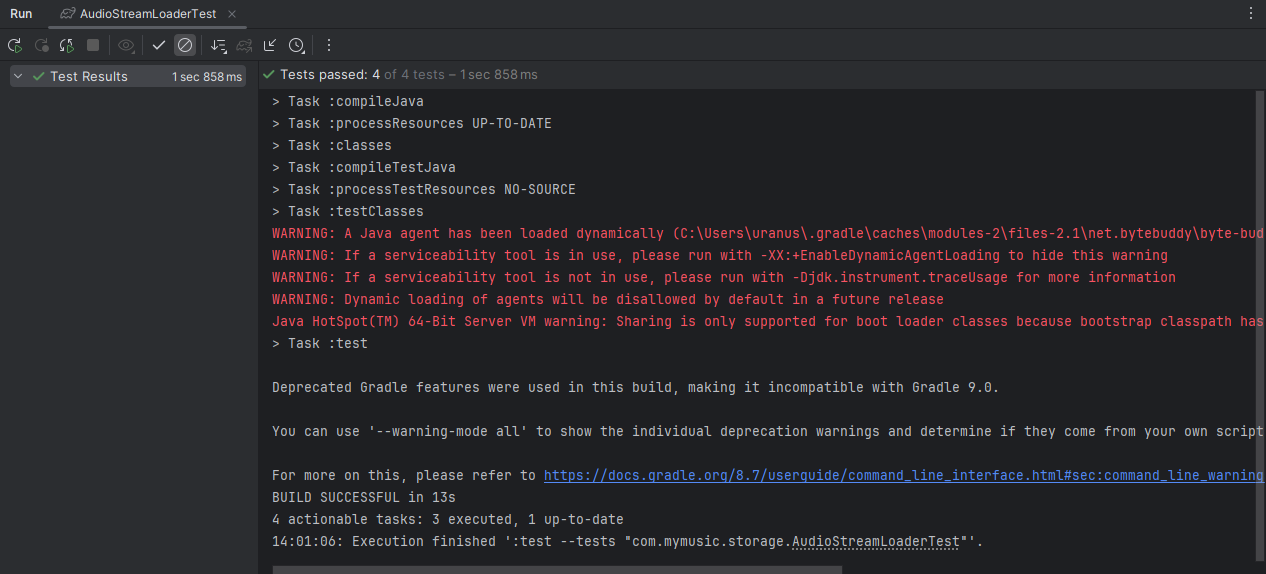
\includegraphics[width=0.8\linewidth]{unitASLSuc}}
	\caption{Результат успешного прохождения тестов для класса AudioStreamLoaer}
	\label{unitASLSuc:image}
\end{figure}
На рисунках \ref{unitJwt:image}-\ref{unitJwtvalid:image} представлены листинги модульныех тестов для модуля генерации Jwt токенов JwtTokenProvider.
\begin{figure}[!ht]
	\begin{lstlisting}[language=Java]
		class JwtTokenProviderTest {
			@Mock
			private User user;
			@Mock
			private CustomUserDetails userDetails;
			private JwtTokenProvider jwtTokenProvider;
			private final String SECRET = "mysecretkeymysecretkeymysecretkeymysecretkey";
			private final long ACCESS_EXPIRATION_IN_SEC = 3600;
			private final long REFRESH_EXPIRATION_IN_SEC = 86400;
			@BeforeEach
			void setUp() {
				MockitoAnnotations.openMocks(this);
				jwtTokenProvider = new JwtTokenProvider(SECRET, ACCESS_EXPIRATION_IN_SEC, REFRESH_EXPIRATION_IN_SEC);
			}
			@Test
			void generateAccessToken_ShouldGenerateValidToken() {
				when(user.getUserId()).thenReturn(1L);
				when(user.getRole()).thenReturn("USER");
				String token = jwtTokenProvider.generateAccessToken(user);
				assertNotNull(token);
				Claims claims = Jwts.parserBuilder().setSigningKey(SECRET).build().parseClaimsJws(token).getBody();
				assertEquals("1", claims.getSubject());
				assertEquals("USER", claims.get("ROLE"));
			}
			// Другие тесты	
		}
	\end{lstlisting}  
	\caption{Настройка и модульный тест generateAccessToken\_ShouldGenerateValidToken() класса JwtTokenProvider}
	\label{unitJwt:image}
\end{figure}
\begin{figure}[!ht]
	\begin{lstlisting}[language=Java]
		@Test
		void generateRefreshToken_ShouldGenerateValidToken() {
			when(user.getUserId()).thenReturn(1L);
			when(user.getRole()).thenReturn("USER");
			String token = jwtTokenProvider.generateRefreshToken(user);
			assertNotNull(token);
			Claims claims = Jwts.parserBuilder().setSigningKey(SECRET).build().parseClaimsJws(token).getBody();
			assertEquals("1", claims.getSubject());
			assertEquals("USER", claims.get("ROLE"));
		}
	\end{lstlisting}  
	\caption{Модульный тест generateRefreshToken\_ShouldGenerateValidToken() класса JwtTokenProvider}
	\label{unitJwtRef:image}
\end{figure}
\begin{figure}[!ht]
	\begin{lstlisting}[language=Java]
@Test
void generateRefreshToken_ShouldGenerateValidToken() {
	when(user.getUserId()).thenReturn(1L);
	when(user.getRole()).thenReturn("USER");
	String token = jwtTokenProvider.generateRefreshToken(user);
	assertNotNull(token);
	Claims claims = Jwts.parserBuilder().setSigningKey(SECRET).build().parseClaimsJws(token).getBody();
	assertEquals("1", claims.getSubject());
	assertEquals("USER", claims.get("ROLE"));
}
	\end{lstlisting}  
	\caption{Модульный тест generateRefreshToken\_ShouldGenerateValidToken() класса JwtTokenProvider}
	\label{unitJwtRef:image}
\end{figure}
\begin{figure}[!ht]
	\begin{lstlisting}[language=Java]
@Test
void isValid_ShouldReturnTrueForValidToken() {
	when(user.getUserId()).thenReturn(1L);
	when(user.getRole()).thenReturn("ROLE_USER");
	String token = jwtTokenProvider.generateAccessToken(user);	
	assertTrue(jwtTokenProvider.isValid(token, user));
}
	\end{lstlisting}  
	\caption{Модульный тест isValid\_ShouldReturnTrueForValidToken() класса JwtTokenProvider}
	\label{unitJwtvalid:image}
\end{figure}
\begin{figure}[!ht]
	\begin{lstlisting}[language=Java]
		@Test
		void isValid_ShouldReturnFalseForInvalidToken() {
			when(userDetails.getUser()).thenReturn(user);
			when(user.getUserId()).thenReturn(1L);	
			String token = "invalid.token.here";	
			assertFalse(jwtTokenProvider.isValid(token, user));
		}
	\end{lstlisting}  
\caption{Модульный тест isValid\_ShouldReturnFalseForInvalidToken() класса JwtTokenProvider}
\label{unitJwtinvalid:image}
\end{figure}
\\
Результаты успешного выполнения тестов для класса JwtTokenProvider представлены на рисунке \ref{unitJwtSuc:image}.
\begin{figure}[!ht]
	\center{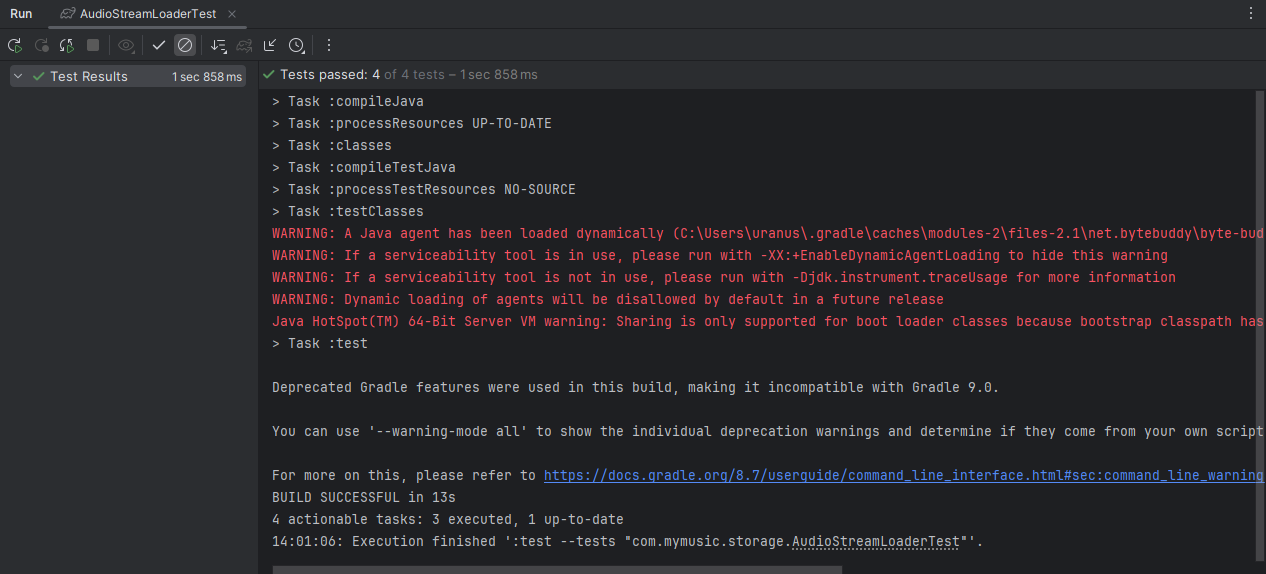
\includegraphics[width=0.7\linewidth]{unitASLSuc}}
	\caption{Результат успешного прохождения тестов для класса JwtTokenProvider}
	\label{unitJwtSuc:image}
\end{figure}


\subsubsection{Системное тестирование}

Системное тестирование является типом тестирования программного обеспечения, направленным на проверку полной интегрированной системы. На этом этапе тестируется вся система в целом, чтобы удостовериться, что все компоненты и модули работают вместе согласно требованиям спецификации. В отличие от модульного тестирования, которое фокусируется на отдельных частях программы, системное тестирование проверяет взаимодействие между различными компонентами и оценивает поведение системы в реальных условиях эксплуатации.
Системное тестирование проводится в среде, максимально приближенной к реальной эксплуатационной среде, что позволяет выявить проблемы, которые могут возникнуть в процессе использования программного обеспечения конечными пользователями.
При входе в web-приложение неаутентифицированного пользователя, ему предлагается войти в систему. Система в данном состоянии представлена на рисунке \ref{stestLoginEmpty:image}.
\begin{figure}[H]
\center{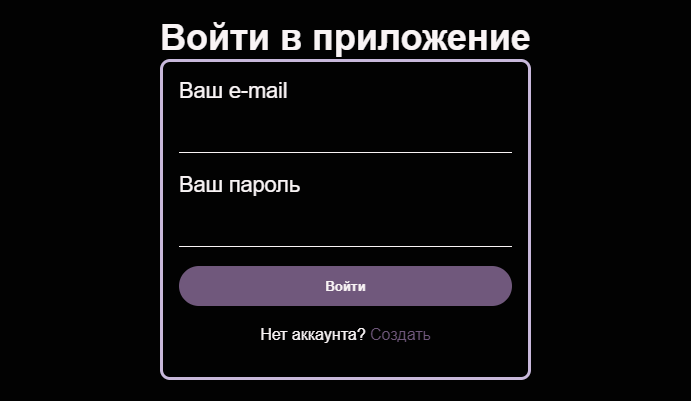
\includegraphics[width=0.8\linewidth]{stestLoginEmpty}}
\caption{Система в состоянии "<Пользователь не аутентифицирован">}
\label{stestLoginEmpty:image}
\end{figure}
В случае наличия аутентификационных данных, пользователь может выполнить вход в систему. В случае отсутствия аутентификационных данных пользователь может перейти на страницу регистрации. Система в состоянии "<Регистрация пользователя"> представлена на рисунке \ref{stestReg:image}.
\begin{figure}[H]
	\center{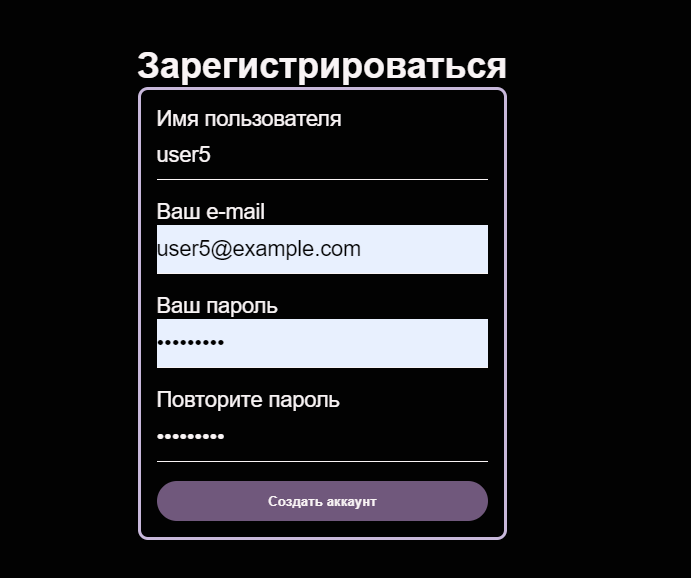
\includegraphics[width=0.8\linewidth]{stestReg}}
	\caption{Система в состоянии "<Регистрация пользователя">}
	\label{stestReg:image}
\end{figure}
После успешной регистрации пользователь вновь попадает на страницу входа, где успешно проходит аутенификацию. После этого пользователь попадает на главную страницу сайта. Данное состояние продемонстрировано на рисунке \ref{stestHome:image}.
\begin{figure}[!htb]
	\center{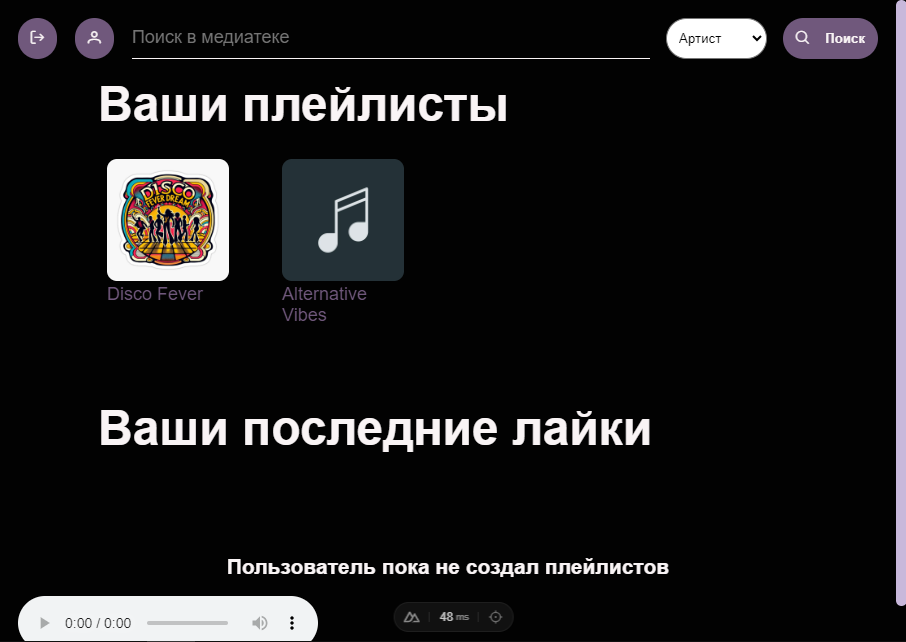
\includegraphics[width=0.8\linewidth]{stestHome}}
	\caption{Система в состоянии "<Главная страница">}
	\label{stestHome:image}
\end{figure}
Пользователь может осуществить поиск контента по строке в одной из категорий: "<артист">, "<альбом"> и "<плейлист">. В случае наличия контента пользователь получит список ссылок. Если же запрашиваемый контент не найден, то пользователь видит соответствующее сообщение. Система в состоянии "Успешный поиск" представлена на рисунке \ref{stestSearchSuc:image}.
\begin{figure}[H]
	\center{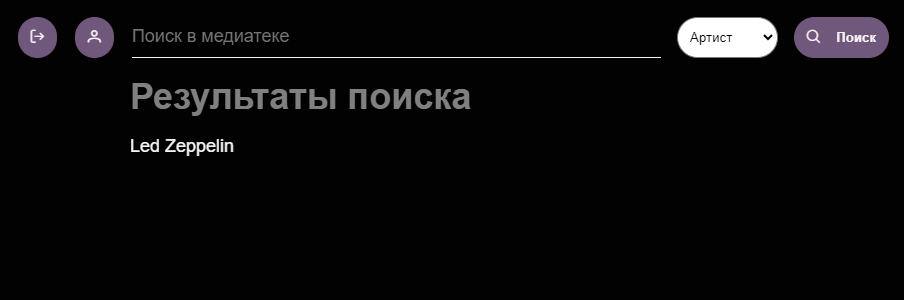
\includegraphics[width=1\linewidth]{stestSearchSuc}}
	\caption{Система в состоянии "<Успешный поиск">}
	\label{stestSearchSuc:image}
\end{figure}
Система в состоянии "<Неудачный поиск"> представлена на рисунке \ref{stestSearchFail:image}.
\begin{figure}[H]
	\center{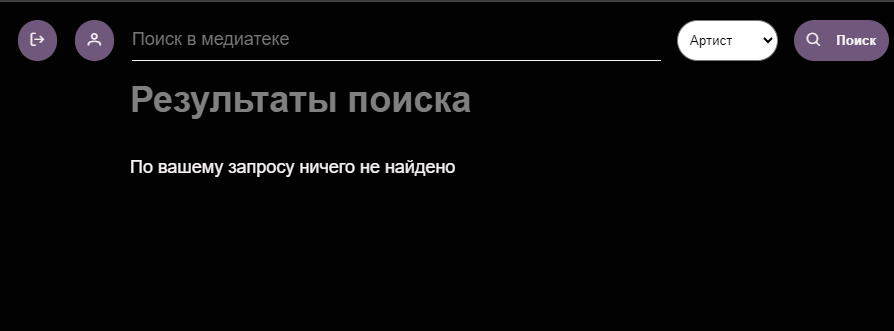
\includegraphics[width=0.9\linewidth]{stestSearchFail}}
	\caption{Система в состоянии "<Неудачный поиск">}
	\label{stestSearchFail:image}
\end{figure}
В случае успешного поиска пользователь может перейти по ссылкам результата поиска. В этом случае пользователь попадает на страницу с контентом, например на страницу артиста. Система в этом состоянии представлена на рисунке \ref{stestArtist:image}.
\begin{figure}[H]
	\center{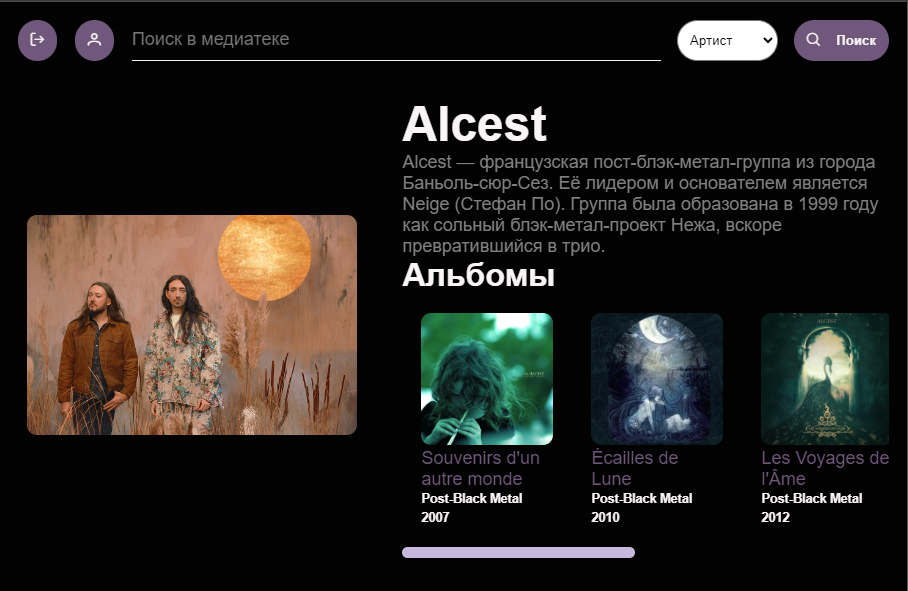
\includegraphics[width=0.8\linewidth]{stestArtist}}
	\caption{Система в состоянии "<Страница артиста">}
	\label{stestArtist:image}
\end{figure}
Пользователь может перейти к одному из альбомов артиста, кликнув по имени альбома. В этом случае пользователь попадает на страницу альбома. Система в этом состоянии представлена на рисунке \ref{stestAlbum:image}.
\begin{figure}[H]
	\center{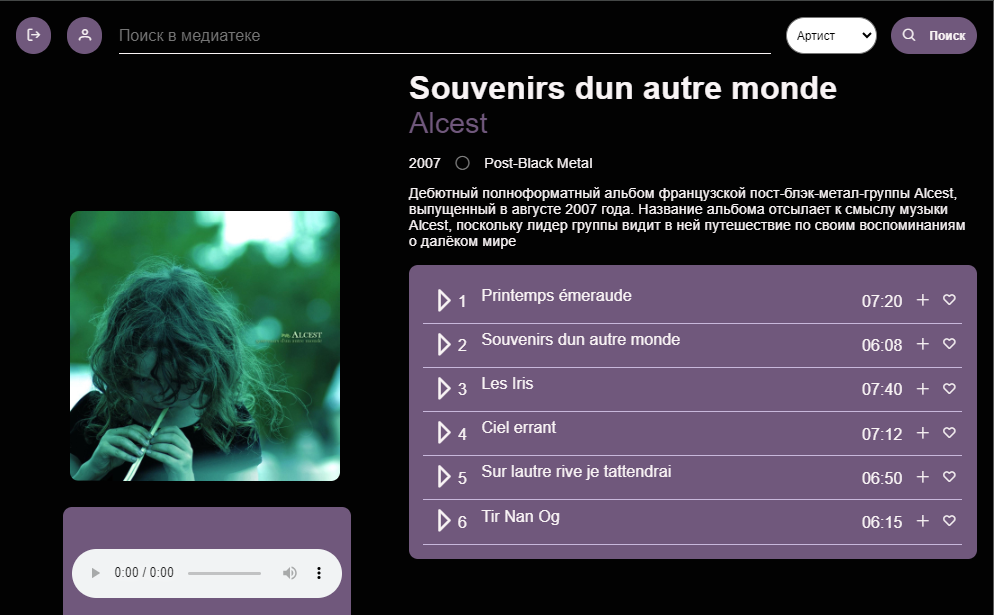
\includegraphics[width=0.8\linewidth]{stestAlbum}}
	\caption{Система в состоянии "<Страница альбома">}
	\label{stestAlbum:image}
\end{figure}
Пользователь может воспроизвести трек, щелкнув по иконке "<играть">. В этом случае плеер внизу экрана отобразит данные трека и начнется воспроизведение трека. Система в этом состоянии отображена на рисунке \ref{stestPlayer:image}.
\begin{figure}[H]
	\center{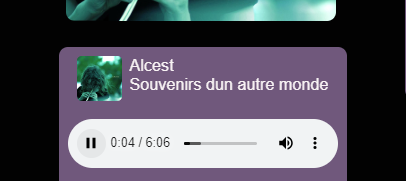
\includegraphics[width=0.8\linewidth]{stestPlayer}}
	\caption{Система в состоянии "<Воспроизведение  трека">}
	\label{stestPlayer:image}
\end{figure}
Пользователь может получить доступ к своей странице. Для этого ему необходимо щелкнуть по кнопке с иконкой пользователя в верхней части приложения. В этом случае откроется страница пользователя. Система в этом состоянии изображена на рисунке \ref{stestUserBefore:image}.
\begin{figure}[H]
	\center{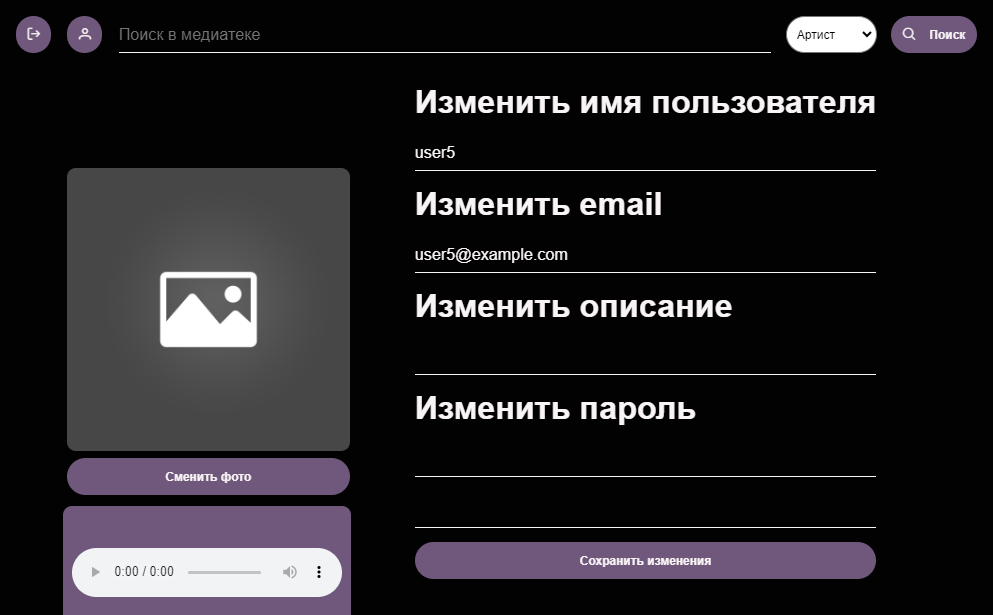
\includegraphics[width=0.8\linewidth]{stestUserBefore}}
	\caption{Система в состоянии "<Страница пользователя">}
	\label{stestUserBefore:image}
\end{figure}
Пользователь может получить изменить данные на своей странице. Для этого ему необходимо ввести новые данные в форме на странице, а затем подтвердить изменения, нажав на кнопку "<Сохранить изменения">. Система в этом состоянии изображена на рисунке \ref{stestUserAfter:image}.
\begin{figure}[H]
	\center{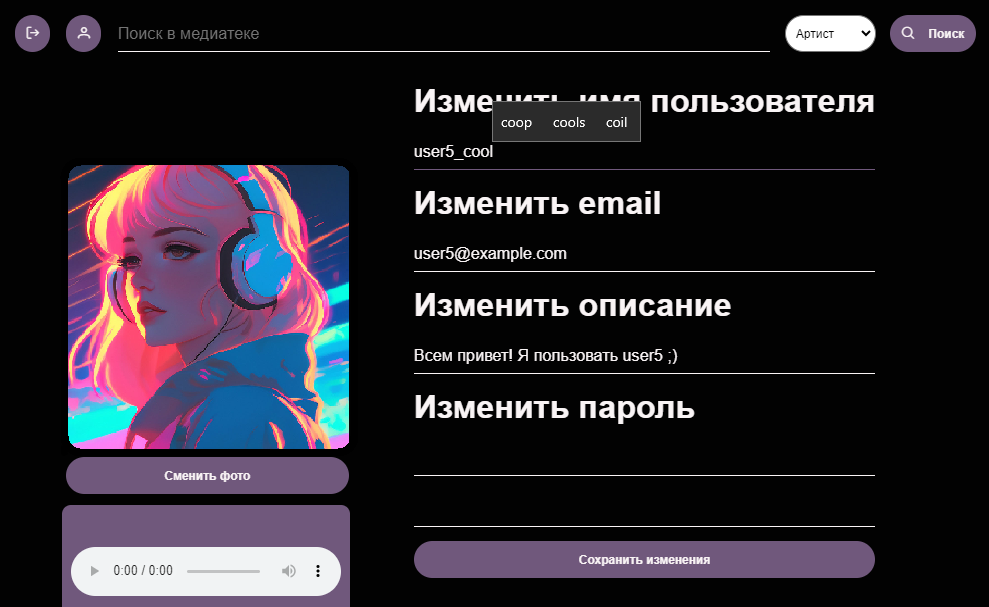
\includegraphics[width=0.8\linewidth]{stestUserAfter}}
	\caption{Система в состоянии "<Изменение данных">}
	\label{stestUserAfter:image}
\end{figure}
\clearpage